
%!TEX encoding = UTF-8 Unicode
\documentclass{simpleslides}

\author{Björn Regnell \\ \vspace{1em}{\small \url{https://cs.lth.se/bjorn-regnell}}}
\title{An Overview of Selected\\Requirements Engineering Methods}

\date{\footnotesize Version: \today}
\begin{document}
\maketitle

\begin{frame}[fragile]{Requirements Elicitation Methods}
\begin{itemize}
\item Stakeholder analysis
\item Interviews
\begin{itemize}
  \item Unstructured interviews: open questions, open topics
  \item Structured interviews: closed questions, focused topics
  \item Semi-structured: combine both
\end{itemize}
\item Surveys
\item Group activities
\begin{itemize}
  \item Brainstorming -- generate ideas, creativity games
  \item Focus groups -- gather a group of stakeholders
  \item Demonstrations -- work enactment in a usage context
\end{itemize}
\item Usability testing
\item Usage statistics
\item Feedback from marketing and support
\item User and developer communities
\item Mining social media
\end{itemize}
\small  Some methods are good for both elicitation and validation, e.g:\\
focus groups, usability testing
\end{frame}
  

\begin{frame}[fragile]{Requirements Specification Methods}
Different kinds of representations:
\begin{itemize}
\item Text, photos, drawings, diagrams, movies, prototypes, ...
\end{itemize}
Examples of requirements models:
\begin{itemize}
\item Static models: What exists in the domain and product?
\begin{itemize}
\item Goal models: stakeholders, goals+relations (helps, hurts)
\item System scope: context diagram, actors, interfaces
\item Data models: E/R-diagrams, Data dictionaries
\item Feature models (in text or pictures):\\why, what: functions+data, examples of how,\\expected quality,\\links to other features and models
\end{itemize}
\item Dynamic Models: What happens at runtime?
\begin{itemize}
\item Scenario-based models:\\narratives, user stories, task models, use case models
\item State-transition models: state diagrams, transition matrices
\item Test Cases: acceptance tests, system tests, unit tests
\item User interface models: mockups, GUI Designs
\item Communication protocols
\end{itemize}
\end{itemize}
\end{frame}

\begin{frame}[fragile]{Context Diagram}
\begin{itemize}
\item A context diagram depicts the domain in terms of external entities (actors) that interact with the system via interfaces
\item The system under development is a ''black box'', no internal structure is shown -- it is the context that is in focus
\item Often only includes the inner domain (direct actors) and not the outer domain (indirect actors)
\item Interfaces are named and linked to specifications of data requirements, protocols, GUI prototypes
\end{itemize}
\end{frame}

\begin{frame}[fragile]{Specificy features by mixed levels of abstraction}
You can use several parts of the Goal-Design scale when you specify a feature:
  \begin{itemize}
\item \textbf{Goal-level}: provide the rational of \emph{why} this feature is needed, link to goal model 
\item \textbf{Domain-level}: describe a usage context and how the feature is used, both normal and exceptional usage, variants, domain-level events, etc.
\item \textbf{Product-level}: describe the input-output relation, normal and exceptional input/output, product-level events, etc.
\item \textbf{Design-level}: give examples and expectations but often best to explicitly state that they are \emph{only} examples; you don't want to constrain the solution space too hard
\end{itemize}
If you want to only specify some of these levels, it is often most valuable to select the \textbf{higher} rather than the lower levels, in terms of reducing the risk of implementing the wrong features.
\end{frame}

\begin{frame}[fragile]{Scenario-based requirements}
\begin{itemize}
  \item User stories
  \item Task descriptions
  \item Use cases
  \item Narrative scenarios
\end{itemize}
\end{frame}

\begin{frame}[fragile]{Specifying Quality Requirements}
\begin{itemize}\small
\item Which quality requirements should we specify? \\ {\footnotesize 
accuracy, capacity, performance, reliability, security, safety, maintainability, usability, ... }
\item Challenges:
\begin{enumerate}\footnotesize
\item can be system-wide or specific to a function
\item can be fulfilled to a certain degree on a sliding scale
\item a measurement scale can be difficult to define
\item can be difficult to measure and select targets (is it feasible?)
\item sometimes subjective in the view of a certain stakeholder
\item quality aspects are often mutually dependent and overlapping,\\
      example: usability depends on performance and reliability
\item quality aspects may be conflicting, examples: \\ higher security may mean lower usability, \\ higher performance may mean lower maintainability
\end{enumerate}
\item Approaches:
\begin{itemize}\footnotesize
\item Define a \textbf{scale} and set a \textbf{target} in a context with a \textbf{margin}
\item Prioritize which aspects are more \textbf{important} than others
\item Leave undecided aspects \textbf{open} to the supplier/developer:
\item[] \textbf{Open target}: Define a scale but leave value open (+ expectation)
\item[] \textbf{Open metric}: Leave the scale open
\item Quality aspects can often be turned into functionality,\\
      example: a security goal lead to a login function
\end{itemize}
\end{itemize}
\end{frame}


\begin{frame}[fragile]{Requirements Validation Methods}
Things to check:
\begin{itemize}\small
\item The quality of your requirements models:\\correct, unambiguous, complete, consistent, concise, comprehensible, verifiable, feasible, traceable, modifiable...  
\item Checking each representation in isolation
\item Checks of consistency among representations
\item Check rationale (goals, domain-level information, why?)
\end{itemize}
  
Methods for checking requirements:
\begin{itemize}\small
\item Inspections -- humans inspect (read) models
\item Checklists  -- common mistakes, important checks
\item Automated checks -- tool support
\item Prototyping -- proof-of-concept to validate feasibility
\item Usability testing  -- find real or proxy users, use prototype
\item Focus groups  -- gather a group of stakeholders
\item Simulation -- event-based or continuous model, statistics
\end{itemize}
\end{frame}
  
\begin{frame}[fragile]{Specifying Usability}
Aspects of usability (user experience, UX):
\begin{itemize}
\item It is easy to learn how to use the system
\item I can efficiently carry out my tasks
\item I can easily remember how to use the system
\item I can understand what I need to do and what happens (clear mental model)
\item I like it! (subjective satisfaction, great user experience)
\end{itemize}
Some approaches to specification:
\begin{itemize}
\item Characterize max level of usability problems per time unit
\item Characterize task efficiency, given user experience level 
\item Require minimum results in user surveys on satisfaction 
\item Design and prototype a UI and usability test it
\item Requirements on the development process: ''you have to use prototyping and usability testing like so: ...''
\item Require the the system comply with style guides and usability standards
\end{itemize}

\end{frame}

\begin{frame}[fragile]{Specification by referring to standards}
Sometimes it is suitable to specify requirements on functionality or quality by referring to standards relevant to your domain.
\begin{itemize}
\item Some advantages:
\begin{itemize}
\item [+] Less work:\\the knowledge is already elicited, specified and validated
\item [+] Your specification becomes more concise
\item [+] Accepted quality and functionality standards of the domain gives credibility
\end{itemize}
\item Some disadvantages:
\begin{itemize}
\item [-] False sense of security:\\ standards might be ambiguous, incomplete, ...
\item [-] The standard may be ''over-kill'', difficult to understand
\item [-] All or nothing if you want to claim compliance:\\can imply many more requirements that also needs to be implemented
\end{itemize}
\end{itemize}
\end{frame}

\begin{frame}[fragile]{Requirements Selection Methods}
\begin{itemize}
\item Software development is an on-going decision process that is enacted throughout the product lifecycle.
\item What is in and what is out at this particular point in time?
\item Methods:
\begin{itemize}
  \item Prioritization
  \begin{itemize}
\item assessing value and cost, making trade-offs
\item volatility assessment
\item risk assessment
\item technical debt assessment
\end{itemize}
\item Road-mapping: long-term product strategy 
\item Release planning: delivery commitments under constraints
\item Being adaptable to changes in plans and strategies
\end{itemize}
\end{itemize}
\end{frame}



\begin{frame}[fragile]{Requirements Prioritization}

\begin{itemize}
\item Examples of different aspects to rank on some scale
\begin{itemize}
  \item value: financial benefit, urgency, strategic value, market share, brand fitness, release theme, ...
  \item cost: staff effort, lead time, training, runtime costs, ... 
  \item volatility: rate of change, uncertainties, ...
  \item risk: technical risk, market risk, competence risk, ...
  \item ...
\end{itemize}
\item Different types of scales with different power
\begin{itemize}
  \item categorization \{A, B\}: must, ambiguous, volatile
  \item ordinal scale $A > B$: higher value, more expensive 
  \item ratio scale $A = k \cdot B$: amount of money, hours, percentage
\end{itemize}
\item Different methods, can be combined
\begin{itemize}
  \item grouping, e.g. post-it notes on a white-board
  \item select top N, e.g. N=5
  \item grading of singular requirements, e.g. 1..5, high--medium--low 
  \item ordering by pair-wise comparison (sorting)
  \item \$100-test: distribute fictitious money to reflect priority
\end{itemize}
\end{itemize}
\end{frame}

\begin{frame}[fragile]{The QUPER model: prioritizing quality requirements}
\begin{center}
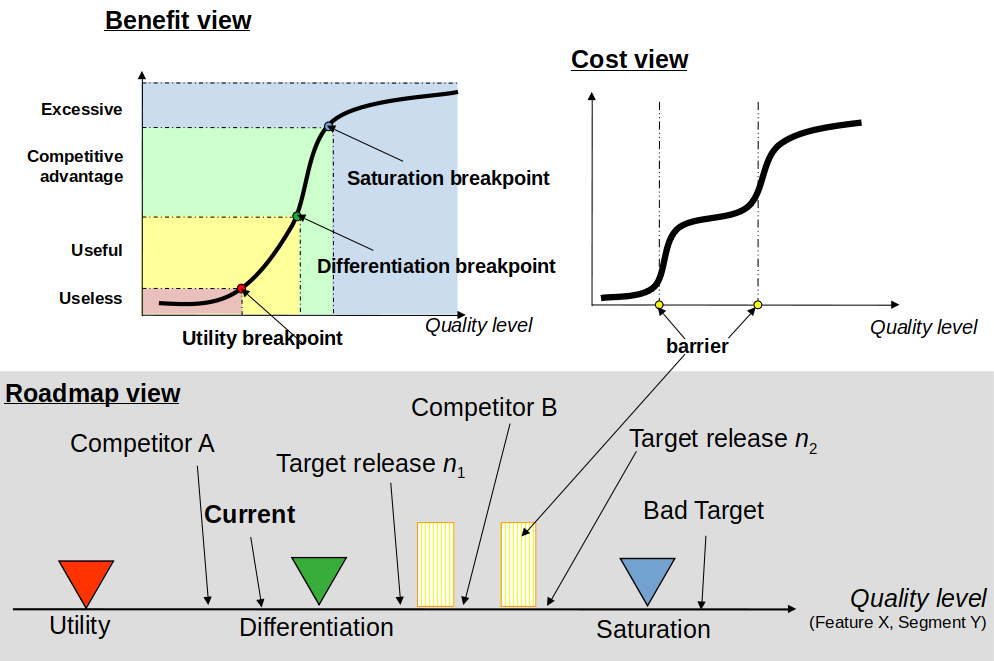
\includegraphics[width=1.0\textwidth]{img/quper}
\end{center}
{\footnotesize ''Supporting Roadmapping of Quality Requirements'' 
\\ B. Regnell, R. Berntsson Svensson, T. Olsson, \emph{IEEE} Software (2008)}
\end{frame}
  

\begin{frame}[fragile]{Written report in Requirements Enigeering}
\begin{itemize}
\item Select a topic of interest
\item Literature search
\item Read selected papers
\item Discuss with peers
\item Write report
\item Get feedback
\end{itemize}
\end{frame}

\begin{frame}[fragile]{Further studies in RE}
  Starting-points for literature search:

\begin{itemize}\footnotesize
\item \url{https://scholar.google.se/} within the \texttt{lu.se} domain
\item \url{https://cs.lth.se/bjorn-regnell/publications/}
\end{itemize}

4 methods to elicit academic papers:
\begin{itemize}\footnotesize
\item By carefully crafted \textbf{search string} in research databases
\item By \textbf{forum}: browse all titles (for selected years) of a certain forum
\item By \textbf{author}: browse all papers by a specific scholar 
\item By \textbf{reference}: follow references (of references) of interesting papers
\end{itemize}

3 academic forums for Requirements Engineering research:
\begin{itemize}\footnotesize
\item \textbf{REFSQ}: Requirements Engineering -- Foundation for Software Quality \\An international conference held in Europe annually, focuses on novelty rather than maturity/prestige; ''you heard it first at REFSQ''
\item \textbf{RE}: Joint International Conf. on Requirements Engineering \\Alternating between Europe, Americas, Asia; a prestigious forum with low acceptance rate
\item \textbf{REJ}: Requirements Engineering Journal by Springer Nature \\ Longer papers with mature results of high credibility. 
\end{itemize}
  
\end{frame}

\begin{frame}[fragile]{Recommended conference: REFSQ2024 April 8--11}
\begin{itemize}
\item I \textbf{sincerely recommend} to visit the REFSQ conference:
\item[] Requirements Engineering:\\Foundation for Software Quality
\item[] 
\item Mon 8 -- Thu 11 April 2024 Winterthur, Switzerland 
\item \textbf{Industry track}: discuss with other RE practitioners
\item[] Contact the industry track chairs if you want to speak or contribute in other ways -- perhaps you want to send a whole group from BorgWarner?
\item \textbf{Research track}: novel methods are investigated
\item [] ''you heard it first at REFSQ''
\item []
\item   \url{https://2024.refsq.org/}
\end{itemize}

\end{frame}

\begin{frame}[fragile]{Recommended literature}
\begin{itemize}\footnotesize%\fontsize{8}{10}\selectfont
\item \textbf{Supporting Roadmapping of Quality Requirements} \\ B. Regnell, R. Berntsson Svensson, T. Olsson, \emph{IEEE} Software (2008) 
\item \textbf{An Industrial Case Study on Distributed Prioritisation in Market-Driven Requirements Engineering for Packaged Software}\\ 
Björn Regnell, Martin Höst, Johan Natt och Dag, Per Beremark, Thomas Hjelm
Requirements Engineering Journal, Springer (2001) 6:51–62
\item \textbf{Requirements engineering challenges in market-driven software development -- An interview study with practitioners} \\ L. Karlsson, Å. G. Dahlstedt, B. Regnell, J. Natt och Dag, A. Persson, \emph{Information and Software Technology} (2008) 
\item \textbf{Market-Driven Requirements Engineering for Software Products} \\ B. Regnell, S. Brinkkemper \\ \emph{Chapter 13 in the book ''Engineering and Managing Software Requirements} Eds. Wholin \& Aurum'',  ISBN 3 540 25043 3 (2005)
\item \textbf{Software Requirements - Styles and Techniques}, Soren Lauesen, Addison--Wesley, ISBN 0-201-74570-4, 2002.
\end{itemize}
\end{frame}



\end{document}

